\documentclass{article}
\usepackage{../repsty}
\usepackage{wrapfig}

\begin{document}

\title{Statistical modeling}
\author{Alexander Aksentyev}
\maketitle

\section*{Introduction}
When determining a double-polarized observable using the transmission-experiment method, one estimates the rate of decay of the beam current. This can be done by fitting a linear model to the log-transformed beam current data using the Ordinary Least Squares method.

The observable ($\A$) can then be estimated as a difference statistic of the slopes in the two appropriate polarization cases, and its variance will be proportional to the sum of the variances of the constituent slope estimates: $\SE{\A*} = C\sqrt{2}\cdot\SE{\slp*}$.

For the mean statistic, its precision depends on the precision of the slope estimate $\SE{\slp*}$ as in
\begin{equation}\label{eq:AvgASE}
	\SE{\avg{\A*}} = \frac{\SE{\A*}}{\sqrt N} = \sqrt{2}\sqrt{\frac hH}\cdot\SE{\A*} = 2C\sqrt{\frac hH}\cdot\SE{\slp*},
\end{equation}
where $H$ is the beam time, $h$ the cycle length, and so the maximum number of estimate pairs $N = \sfrac{H}{2h}$.

The conditions for the OLS estimators of the model parameters belonging to the class of the minimum-variance unbiased estimators are given by the Gauss-Markov theorem. 

Here we will try to estimate the beam and cycle times appropriate for achieving the required precision $\SE{\Ayy*}$ of the cross section asymmetry estimate $\Ayy*$. At first, we will estimate the required beam time under the Gauss-Markov conditions. Then, for the estimation of the appropriate measurement cycle length, we will relax the strict exogeneity condition, by assuming that the slope varies stochastically about some mean value. We do so to account for the fact that at each turn a slightly different number of particles is scattered due to the stochastic nature of scattering alone. (However the approach taken is independent of the reasons for the slope variation.)

\begin{table}
\centering
\caption{Parameter values (June 2016)\label{tbl:Param}}
\begin{threeparttable}[h]
\begin{tabular}{p{4.5cm}llr}
	\hline\hline
	Parameter                                 & Symbol            & Value              &               Dimension \\ \hline
	Beam revolution frequency                 & $\nu$             & 0.79               &                     MHz \\
	Target thickness                          & $\Thick$          & $1.1\cdot 10^{14}$ & $\Dim{at\cdot cm^{-2}}$ \\
	Target polarization                       & $P^t$             & 0.88               &                      -- \\
	Beam spin up-down polarization difference & $\DP$             & 1.48               &                      -- \\
	$pd$ scattering cross section             & $\CS[0]$\tnote{a} & 70                 &                      mb \\ \hline
\end{tabular}
\begin{tablenotes}
	\item[a]{From Particle Data Group \url{http://pdg.lbl.gov/2016/hadronic-xsections/rpp2014-pd_pn_plots.pdf}}
\end{tablenotes}
\end{threeparttable}
\end{table}

\section{Required beam time}
\newcommand{\Tint}{\Delta t}
\DeclareDocumentCommand{\v}{O{}mo}{\sigma^2_{#1}\bkt*{#2\IfValueT{#3}{|~ #3}}}

Under the Gauss-Markov conditions, the slope estimate's standard error is
\begin{equation}\label{eq:SlpVarGM}
	\SE{\slp*} = \frac{\SE{\err}}{\sqrt{\sum_{k=1}^K (t_k - \avg{t})^2}},
\end{equation}
where $\SE{\err}$ is the measurement resolution, $K$ is the sample size, and $t_k$ is the measurement time.

Since the measurements are taken uniformly in time with step $\Tint$, rewriting eq.~\eqref{eq:SlpVarGM} in physical terms gets:
\begin{align*}
	\sum_{k=1}^K (t_k - \avg{t})^2 &= \sum_k \bkt{k\Tint - \frac{1}{K}\sum_{k=1}^K k\Tint}^2; \\
	\frac{1}{K}\sum_{k=1}^K k\Tint  &= \frac{\Tint}{2}(K+1)\equiv \Tint\mu, \\
	\sum_k (k\Tint - \mu\Tint)^2 	&= \Tint^2\sum_k\bkt{
											k^2 - 2k\mu + \mu^2
										} \\
									&= \Tint^2\bkt{\sum_k k^2 - 2\mu\sum_k k + \mu^2K} \\
									&= \Tint^2\bkt{
											\frac{2K+1}{3}K\mu - 2\mu^2K + \mu^2K
										} 
		 							 = \Tint^2\mu K\bkt{\frac{2K+1}{3} - \mu} \\
									&= \Tint^2\mu K \frac{K-1}{6} \\
									&= \frac{\Tint^2}{12}K(K^2-1),
\shortintertext{and hence}									
	\sqrt{\sum_{k=1}^K(t_k - \avg{t})^2} = \frac{\Tint}{2\sqrt{3}}\sqrt{K}\sqrt{K^2-1}.
\end{align*}
As the number of measurements grows, $K \gg 1$, $K^2-1\approx K^2$, and so
\[
	\sqrt{\sum_k (t_k - \avg{T})^2} \approx \frac{\Tint}{2\sqrt{3}}K\sqrt{K}.
\]

The number $K$ of measurements that go into evaluating a slope is related to the state time $h$ as $K\Tint = h$, hence
\[
	\sqrt{\sum_{k=1}^K (t_k - \avg{t})^2} \approx \frac{h\sqrt{h}}{2\sqrt{3}\sqrt{\Tint}}.
\]
Finally, for the slope variance,
\begin{equation}\label{eq:SlpVar}
	\SE{\slp*} = 2\sqrt{3}\sqrt{\frac{\Delta t}{h}}\frac{\SE{\err}}{h}.
\end{equation}

By plugging it in eq.~\eqref{eq:AvgASE} ($\A* \equiv \Ayy*$) we get
\begin{equation}\label{eq:AvgAyySEPhys}
\SE{\avg{\Ayy*}} = 4\sqrt{3}C\cdot \frac{\sqrt{\Tint}}{h\sqrt{H}}\cdot\SE{\err}.
\end{equation}
The estimated beam time for different values of measurement resolution and precision, computed for the case of 15-minute cycles, is shown in Figure~\ref{fig:BeamTime}.

\begin{figure}[h]
	\centering
	\begin{minipage}{.5\textwidth}
		\centering
		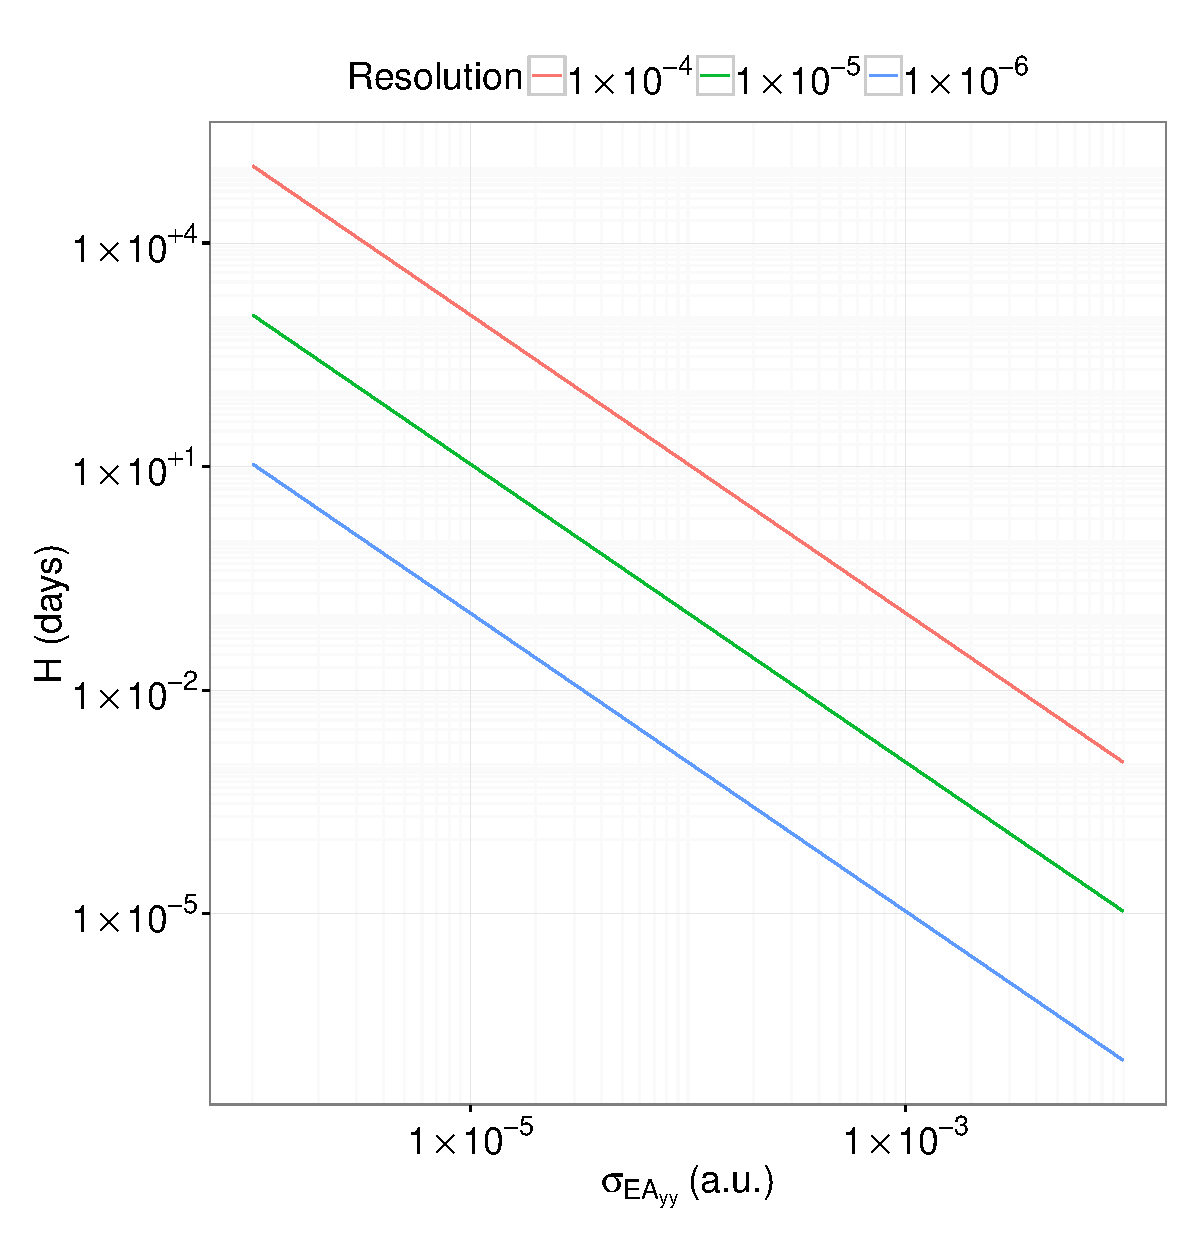
\includegraphics[scale=.5]{BeamTime_15minCycles}
		\caption{Beam time (in full days) as a function of the standard error of the mean $\Ayy$ estimate, required in the case of 15-minute cycles.\label{fig:BeamTime}}
	\end{minipage}~~~~ %
	\begin{minipage}{.5\textwidth}
		\centering
		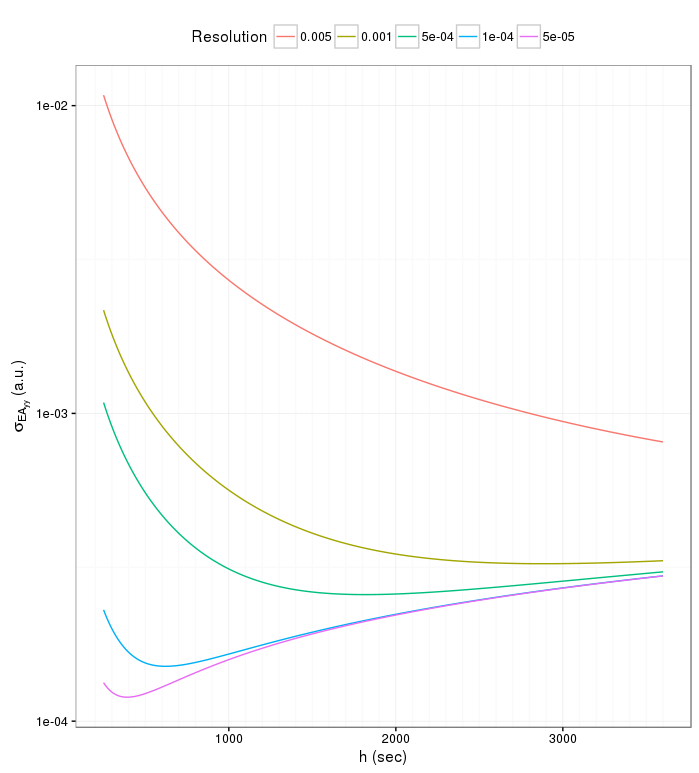
\includegraphics[scale=.5]{SEAyy_varB_15min}
		\caption{The standard error of the mean $\Ayy$ estimate as a function of cycle length when the inherent slope variation $\v{\slp} = 1\cdot10^{-15}$.\label{fig:SEAyy_varb}}
	\end{minipage}

\end{figure}

\section{Appropriate cycle length}
\DeclareDocumentCommand{\Xpct}{O{}mo}{\mathrm{E}_{#1}\bkt*{#2\IfValueT{#3}{|~ #3}}}
Suppose the slope varies; in that case the law of total variance says that 
\begin{equation}\label{eq:VarSlpLTV}
	\v{\slp*} = \Xpct[\slp]{\v{\slp*}[\slp]} + \v[\slp]{\Xpct{\slp*}[\slp]}.
\end{equation}
\begin{align*}
\Xpct{\slp*}[\slp] 	&= \slp, \\
\v{\slp*}[\slp] 	&= 12\frac{\Tint}{h}\frac{\v{\err}}{h^2}, \tag{eq.~\eqref{eq:SlpVar}}
\shortintertext{and hence}
\v{\avg{\Ayy*}}		&= \frac{4 C^2}{H}\bkt{12\Tint\cdot\frac{\v{\err}}{h^2} + h\cdot\v{\slp}}.
\end{align*}
The first term describes the estimate's statistical precision, the second its accuracy. By decreasing the cycle length we reduce precision, but improve accuracy. The accuracy is improved simply by virtue of better averaging of $\v{\slp}$.

The slope variation determines the best achievable precision (see Table~\ref{tbl:SEAyy_varb}). From the last expression, the best variance is achieved at
\begin{equation}
	h_{best} = \sqrt[3]{24\cdot \Tint} \bkt{\frac{\v{\err}}{\v{\slp}}}^{1/3}.
\end{equation}

\begin{table}[h]
\centering
\caption{Best achievable precision of $\Ayy*$,\\ and the corresponding cycle time.\label{tbl:SEAyy_varb}}
\begin{tabular}{lrr}
\hline\hline
$\SE{\err}$			&	$h_{best}$ (min)	& $\SE{\avg{\Ayy*}}$\\
\hline
$5\cdot10^{-3}$		&	141					& $8\cdot10^{-4}$\\
$1\cdot10^{-3}$		&	48					& $3\cdot10^{-4}$\\
$5\cdot10^{-4}$		&	30					& $3\cdot10^{-4}$\\
$1\cdot10^{-4}$		&	10					& $2\cdot10^{-4}$\\
$5\cdot10^{-5}$		&	7					& $1\cdot10^{-4}$\\
\hline
\end{tabular}
\end{table}

\subsection{Inherent slope variation}
By definition, the slope at time $t$ is
\[
 \slp[t] = \frac{\Delta \ln I_t}{\Delta t} \approx \frac{1}{\Delta t}\frac{\Delta I_t}{I_t} \propto \frac{\Delta N_t}{N_t}, ~\Delta N_t \sim B(N_t, p),
\]
where $N_t$ is the number of beam particles at time $t$, $p$ is the probability to scatter a particle, and $B$ refers to the binomial distribution.

Since this is a sample proportion, 
\begin{equation*}
\begin{cases}
	\Xpct{\slp[t]} 	&= p, \\
	\SE{\slp[t]}		&= \frac{1}{\Delta t}\frac{\sqrt{p(1-p)}}{\sqrt{N_t}}, \\
	p 				&= \nu\CS[0]\Thick\Delta t.
\end{cases}
\end{equation*}

Again, from the definition
\[
	N_t = N_{t-1}\bkt{1 + \slp[t-1]\Delta t}.
\]

Therefore, 
\begin{equation}
\v{\slp[t]} = \frac{\alpha}{N_t} = \v{\slp[t-1]}\bkt{1 + \slp[t-1]\Delta t}^{-1},
\end{equation}
where, for the parameters of Table~\ref{tbl:Param}, $\v{\slp[0]} \approx 8\cdot10^{-16}$.

\subsection{Effect of target dissipation}
Suppose the target dissipates randomly, at an average rate $r = 10\sfrac{\%}{day} = 1.16\cdot10^{-6}\sfrac{1}{sec}$, and with a standard deviation equal $r$:
\[
	\Thick[t] = \Thick[t-1](1-\alpha_t),~ \alpha_t\sim N(r,r).
\]

Then the slope
\[
	\slp[t] = \nu\CS[tot]\Thick[t] = \slp[0]\prod_{i=1}^{t-1}(1-\alpha_i),
\]	
and we can estimate $\bkt{\v{\slp}}(h) = \sfrac 1h \sum_{i=1}^{h}(\slp[i] - \avg{\slp})^2$. As one can see from Figure~\ref{fig:varB_TD}, the variance doesn't exceed $1\cdot10^{-16}$, thus validating our estimates.

\begin{figure}[h]
\centering
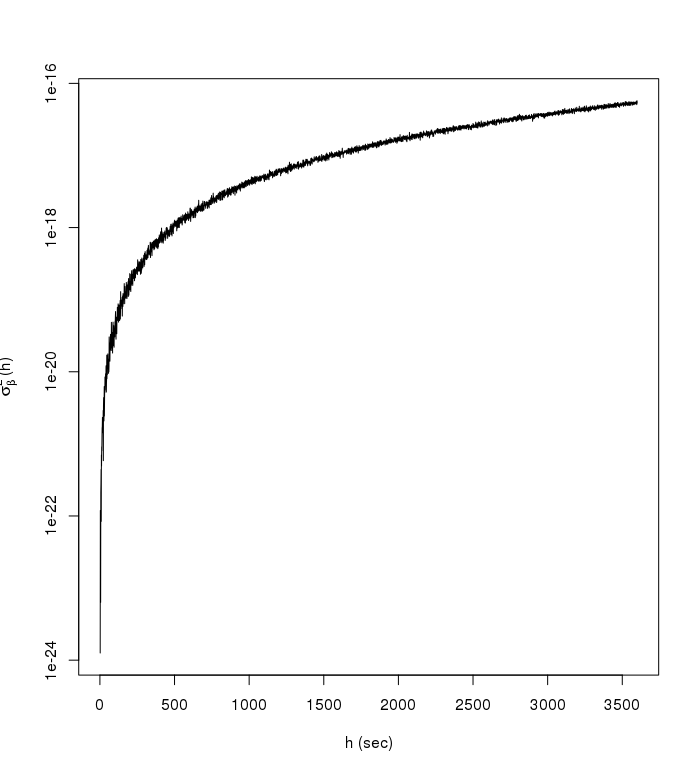
\includegraphics[scale=.5]{varB_DissipThick}
\caption{The growth of the slope dispersion due to a stochastic target dissipation.\label{fig:varB_TD}}
\end{figure}

\end{document}